% !TeX root = ../../ZF_bmicha_Ana.tex
\subsection{Arbeit}
    \vspace{-0.5em}
    \begin{align*}
        W &= \int_C \vec{v} \ d \vec{r} &\textrm{Allgemein}\\
        W &= \int_C \vec{v} (\vec{r}(t)) \cdot \dot{\vec{r}}(t) \ dt &\textrm{Parametr.}\\
        W &= \iint_{A} \textrm{rot}(\vec{v}) \cdot \vec{n_0} \ dA & \textrm{Satz von Stokes}\\
        W &= f\left(P_{\textrm{Ende}}\right) - f\left(P_{\textrm{Anfang}}\right) &\textrm{Potentialfeld}
    \end{align*}

    \subsubsection{Satz von Stokes} \label{sec:SatzVonStokes}
        Falls $\vec{v}$ auf ganz $A$ \textbf{definiert} und \textbf{stetig differenzierbar} (\textit{regulär}) ist, gilt
        $$
            \int_{\partial A} \vec{v} \ d \vec{r} = \iint_{A} \text{rot}(\vec{v}) \cdot \vec{n_0} \ dA,
        $$
        wobei $\partial A$ den geschlossenen Rand der Fläche $A$ bezeichnet.
        Der Normaleneinheitsvektor $\vec{n_0}$ auf $A$ beschreibt mit der \textit{Rechte-Hand-Regel} den Umlaufsinn von $\partial A$.

    \subsubsection{Potentialfeld $\vec{v}$ zum Potential $f$ \label{sec:Potentialfeld}}
        Falls der Definitionsbereich $D(f)$ eines \textbf{wirbel\-freien} ($\text{rot}(\vec{v}) \equiv 0$) Vektorfeldes \textbf{einfach zusammenhängend} (EZH) ist, nennen wir es \textit{konservativ}:
        \mathbox{
           D(f) \textrm{ EZH }\  \textit{und }\ \text{rot}(\vec{v}) \equiv \vec{0} \quad \Rightarrow \quad \vec{v} = \grad(f).
        }
        $$ 
        \vec{v} = 
        \begin{pmatrix}
            u\\v\\w
        \end{pmatrix}
        =
        \begin{pmatrix}
            f_x\\f_y\\f_z
        \end{pmatrix}
        = \grad(f)
        $$ 

        $$
            f(x,y,z) = \int u \ dx = \int v \ dy = \int w \ dz
        $$
        Die Arbeit zwischen zwei Punkten entspricht der Potentialdifferenz.
        % \mathbox{
        %         $\vec{v}$ Potentialfeld &$\Longrightarrow$ $\text{rot}(\vec{v})=\vec{0}$
        % }
        \begin{empheq}[box=\fbox]{align*}
            \vec{v} \textrm{ Potentialfeld } &\Longrightarrow \text{rot}(\vec{v})=\vec{0}\\
            \vec{v} \textrm{ Potentialfeld } &\Longleftarrow \text{rot}(\vec{v})=\vec{0} \textrm{ \& } D(\vec{v}) = \textrm{ EZH}
        \end{empheq}
    
    \subsubsection{Arbeit Berechnen}
        \vspace{0.5em}
        \resizebox*{0.99\linewidth}{!}{
            \tikzset{every picture/.style={line width=0.75pt}} %set default line width to 0.75pt        
            \begin{tikzpicture}[x=0.75pt,y=0.75pt,yscale=-1,xscale=1]
                \draw   (235,71) .. controls (235,66.58) and (238.58,63) .. (243,63) -- (374,63) .. controls (378.42,63) and (382,66.58) .. (382,71) -- (382,95) .. controls (382,99.42) and (378.42,103) .. (374,103) -- (243,103) .. controls (238.58,103) and (235,99.42) .. (235,95) -- cycle ;
                \draw   (385,136) .. controls (385,131.58) and (388.58,128) .. (393,128) -- (524,128) .. controls (528.42,128) and (532,131.58) .. (532,136) -- (532,160) .. controls (532,164.42) and (528.42,168) .. (524,168) -- (393,168) .. controls (388.58,168) and (385,164.42) .. (385,160) -- cycle ;
                \draw    (305,103) -- (245.25,149.5) ;
                \draw [shift={(243.67,150.73)}, rotate = 322.11] [color={rgb, 255:red, 0; green, 0; blue, 0 }  ][line width=0.75]    (10.93,-3.29) .. controls (6.95,-1.4) and (3.31,-0.3) .. (0,0) .. controls (3.31,0.3) and (6.95,1.4) .. (10.93,3.29)   ;
                \draw    (305,103) -- (458.02,126.69) ;
                \draw [shift={(460,127)}, rotate = 188.8] [color={rgb, 255:red, 0; green, 0; blue, 0 }  ][line width=0.75]    (10.93,-3.29) .. controls (6.95,-1.4) and (3.31,-0.3) .. (0,0) .. controls (3.31,0.3) and (6.95,1.4) .. (10.93,3.29)   ;
                \draw    (463.33,168.07) -- (374.88,200.31) ;
                \draw [shift={(373,201)}, rotate = 339.97] [color={rgb, 255:red, 0; green, 0; blue, 0 }  ][line width=0.75]    (10.93,-3.29) .. controls (6.95,-1.4) and (3.31,-0.3) .. (0,0) .. controls (3.31,0.3) and (6.95,1.4) .. (10.93,3.29)   ;
                \draw    (463.33,168.07) -- (547.46,199.3) ;
                \draw [shift={(549.33,200)}, rotate = 200.37] [color={rgb, 255:red, 0; green, 0; blue, 0 }  ][line width=0.75]    (10.93,-3.29) .. controls (6.95,-1.4) and (3.31,-0.3) .. (0,0) .. controls (3.31,0.3) and (6.95,1.4) .. (10.93,3.29)   ;

                % Text Node
                \draw (260,78) node [anchor=north west][inner sep=0.75pt]   [align=left] {Weg geschlossen?};
                % Text Node
                \draw (430,137) node [anchor=north west][inner sep=0.75pt]    {$\text{rot}(\vec{v}) \ \overset{?}{\equiv} 0$};
                % Text Node
                \draw (210,155) node [anchor=north west][inner sep=0.75pt]   [align=left] {Stokes (\ref{sec:SatzVonStokes})};
                % Text Node
                \draw (324,204.5) node [anchor=north west][inner sep=0.75pt]   [align=left] {Potentialfeld (\ref{sec:Potentialfeld})};
                % Text Node
                \draw (512,204.5) node [anchor=north west][inner sep=0.75pt]   [align=left] {Parametrisierung};
                % Text Node
                \draw (250,114.9) node [anchor=north west][inner sep=0.75pt]   [align=left] {Ja};
                % Text Node
                \draw (390,175) node [anchor=north west][inner sep=0.75pt]   [align=left] {Ja};
                % Text Node
                \draw (393,102) node [anchor=north west][inner sep=0.75pt]   [align=left] {Nein};
                % Text Node
                \draw (515,175) node [anchor=north west][inner sep=0.75pt]   [align=left] {Nein};
                % Text Node
                \draw (185,170) node [anchor=north west][inner sep=0.75pt]    {$W = \iint_{A} \text{rot}(\vec{v}) \cdot \vec{n_0} \ dA$};
                % Text Node
                \draw (324,220) node [anchor=north west][inner sep=0.75pt]    {$W = f(P_2) - f(P_1)$};
                \draw (290,235.5) node [anchor=north west][inner sep=0.75pt]    {falls $D(\vec{v})$ einfach zusammenhängend};
                % Text Node
                \draw (496.33,220) node [anchor=north west][inner sep=0.75pt]    {$W = \int_C \vec{v}(\vec{r}(t)) \cdot \dot{\vec{r}}(t) \ dt$};
            \end{tikzpicture}
        }
    